% !TeX root = ../main.tex

\chapter{图表}
\section{插图}
插图功能是利用TeX的特定编译程序提供的机制实现的,不同的编译程序支持不同的图形方式。XeTeX支持插入 EPS、PDF、PNG、JPEG 格式的图片。一般图形都是处在浮动环境中。之所以称为浮动是指最终排版效果图形的位置不一定与源文
件中的位置对应。如果要强制固定浮动图形的位置,请使用float宏包,它提供了 \texttt{[H]} 参数。

\subsection{单个图形}
\begin{figure}[H]
    \begin{center}
        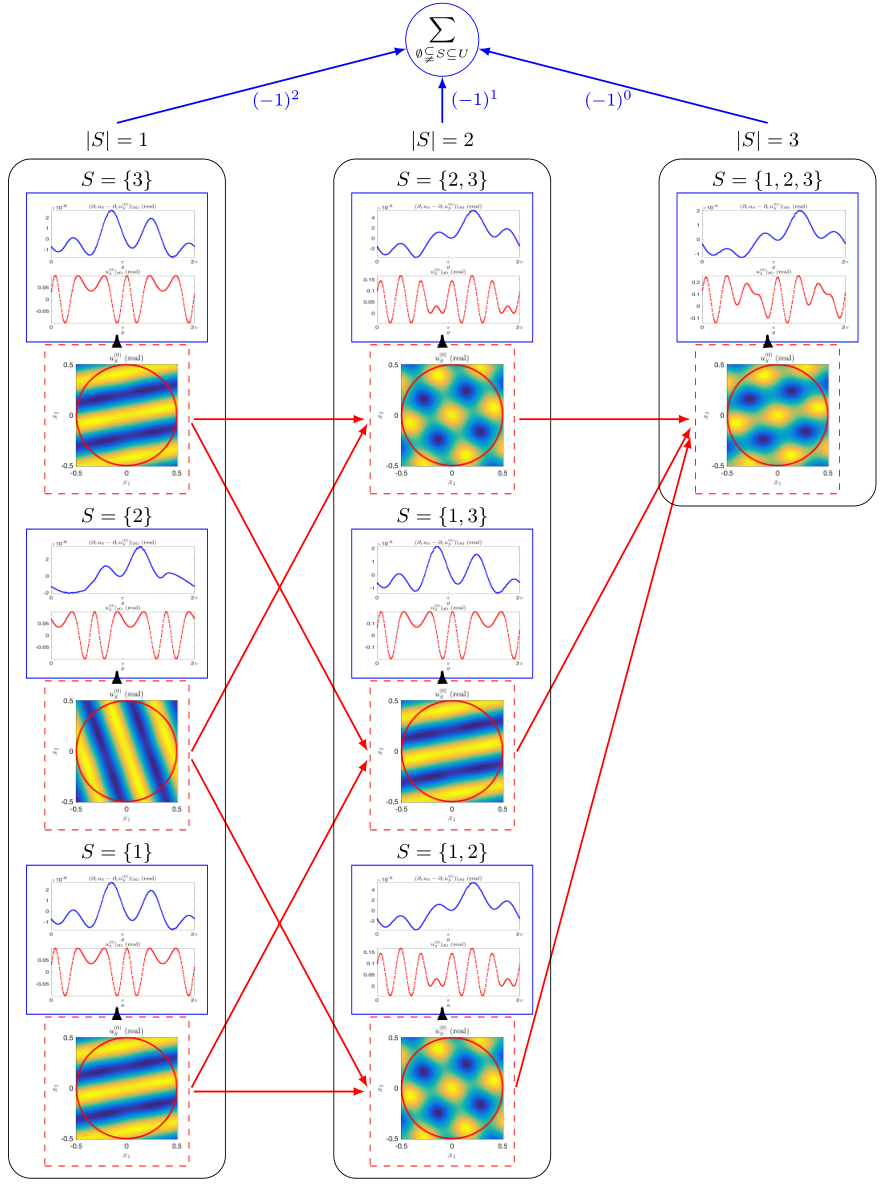
\includegraphics[width=0.5\textwidth]{./figs/cost.png}
\caption[Alessandrini-PIE等式与组合解$u_{S}^{(0)}$]{在非线性次数$m=3$和波数$k=15$时,组合解$u_{S}^{(0)}$的生成.\textbf{红色矩形(虚线)}:$|\xi| = 45.6$时的组合解$u_{S}^{(0)}$.
\textbf{蓝色矩形(实线):} Dirichlet边值 $u_{S}^{(0)} \big|_{\partial\Omega}$ (\textcolor{red}{红色曲线})和线性化Neumann数据的近似$\big( \partial_{\nu} u_{S} - \partial_{\nu} u_{S}^{(0)} \big) \big|_{\partial\Omega}$ (\textcolor{blue}{蓝色曲线}).
\textbf{蓝色圆圈}:根据Alessandrini-PIE等式做组合.}
\label{fig:superposition}
\end{center}
\end{figure}

\subsection{多个图形}
\begin{figure}[H]
\centering
\textbf{非线性次数} $m = 5$ \\[1ex]
\,\hfill \textbf{(i)} $k = 5$ \hfill\,\\
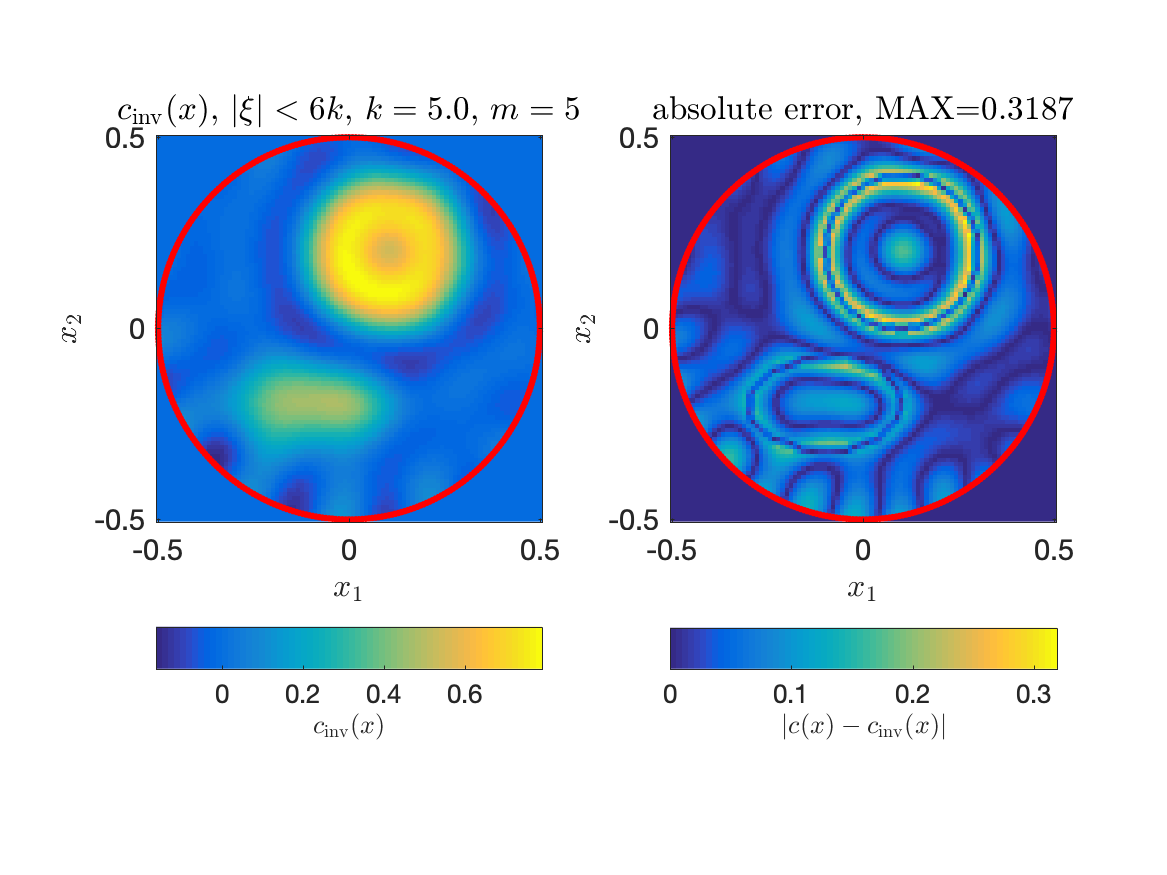
\includegraphics[width=0.45\textwidth,trim=20 60 20 35,clip]{./figs/pwc_5_Ic_0050.png}
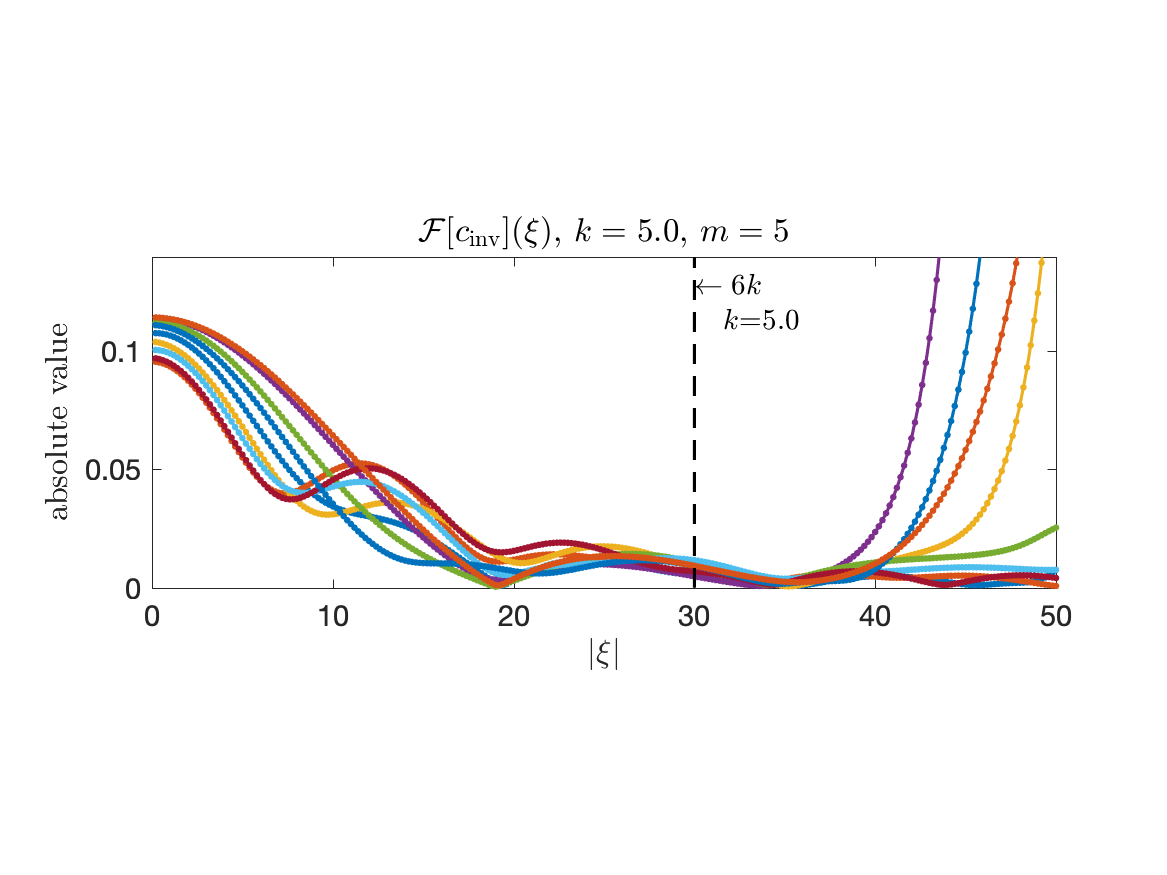
\includegraphics[width=0.54\textwidth,trim=10 60 30 90,clip]{./figs/pwc_5_Fc_0050.png}\\
\,\hfill \textbf{(i)} $k = 10$ \hfill\,\\
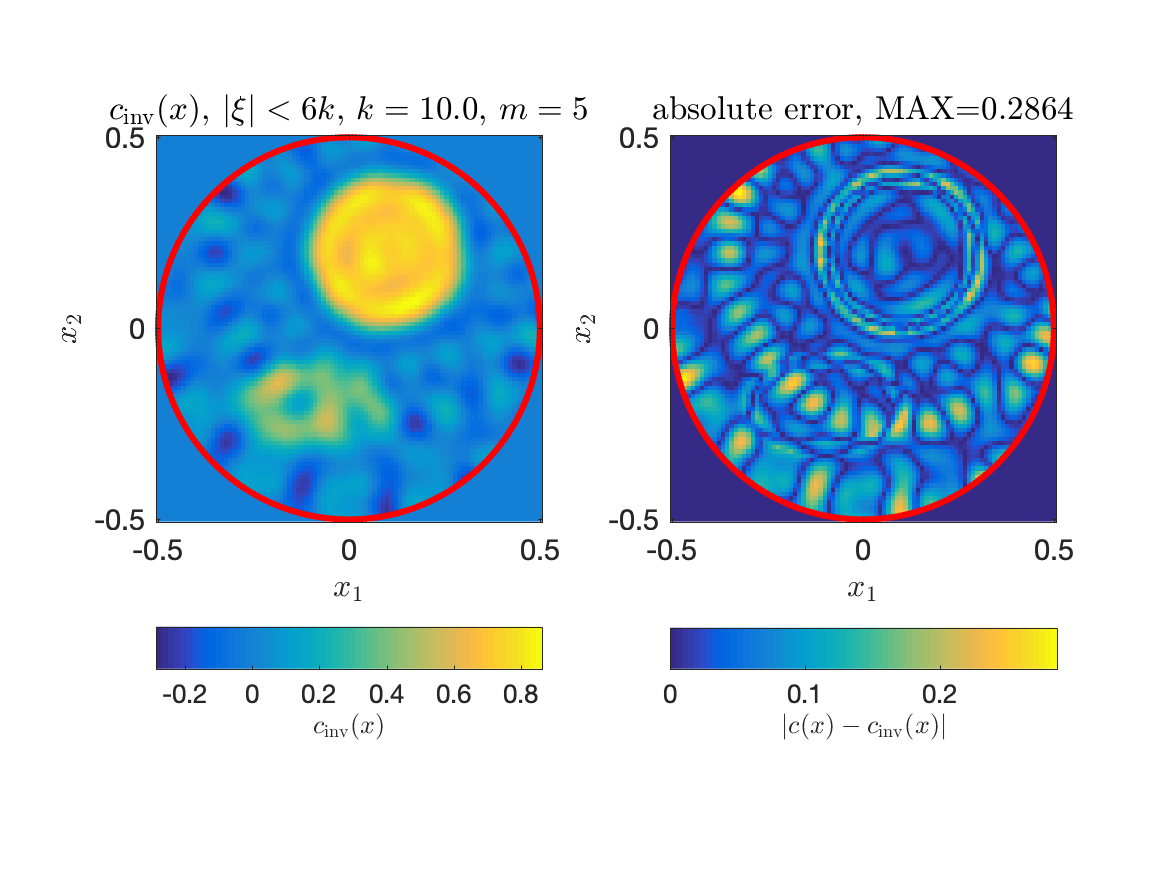
\includegraphics[width=0.45\textwidth,trim=20 60 20 35,clip]{./figs/pwc_5_Ic_0100.png}
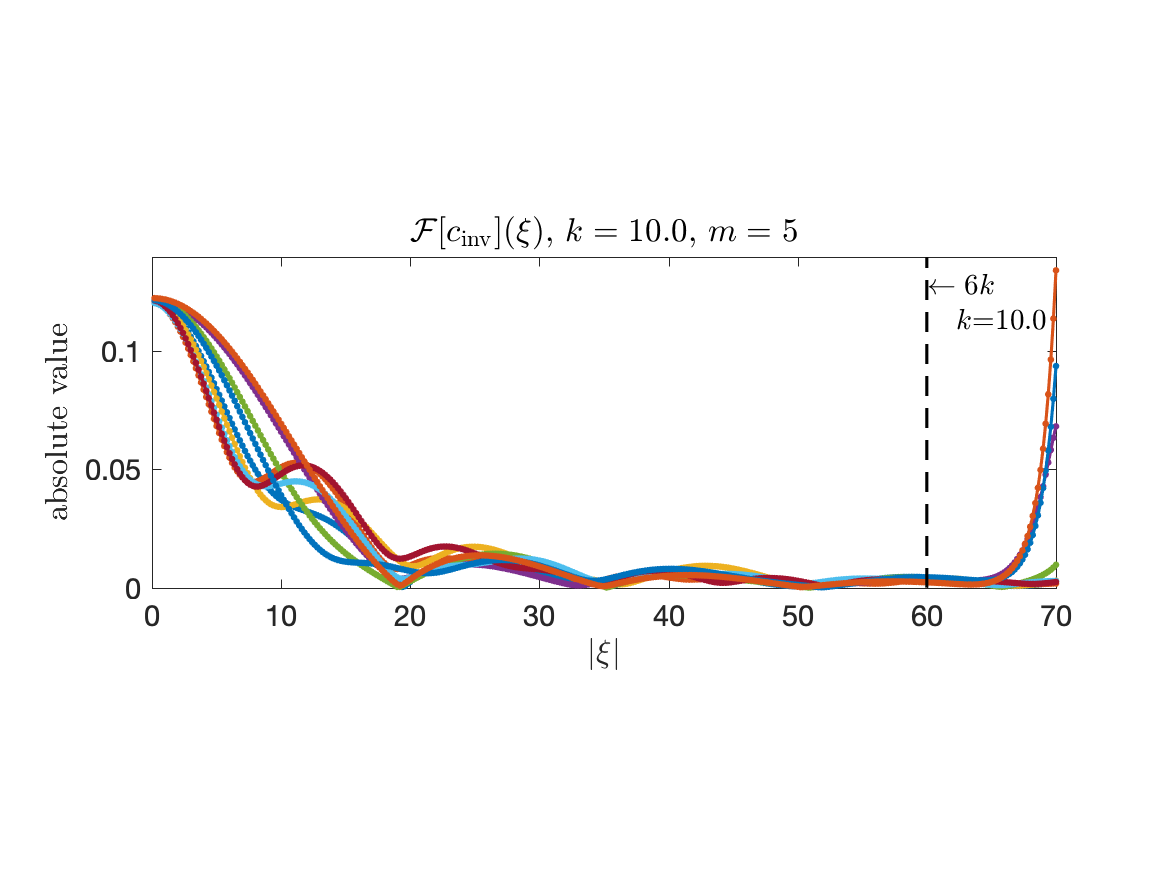
\includegraphics[width=0.54\textwidth,trim=10 60 30 90,clip]{./figs/pwc_5_Fc_0100.png}\\
\,\hfill \textbf{(i)} $k = 15$ \hfill\,\\
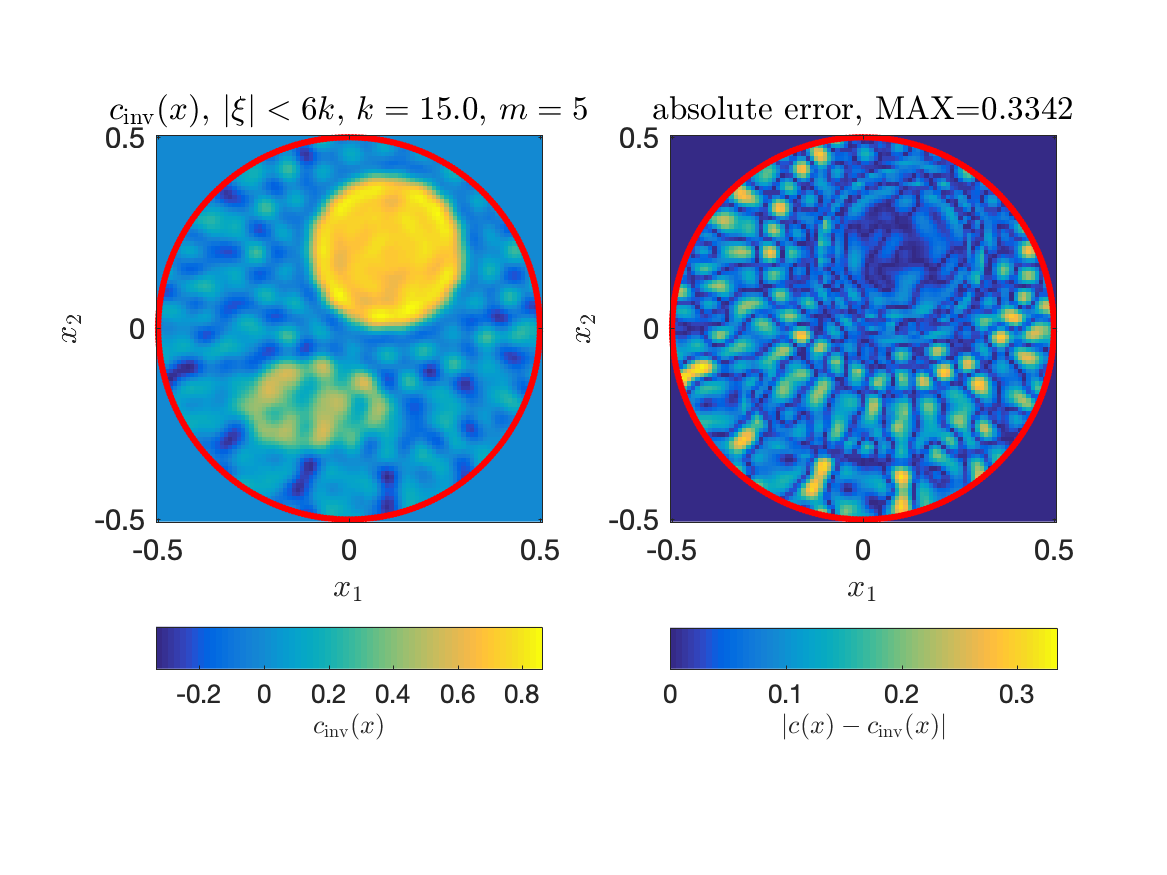
\includegraphics[width=0.45\textwidth,trim=20 60 20 35,clip]{./figs/pwc_5_Ic_0150.png}
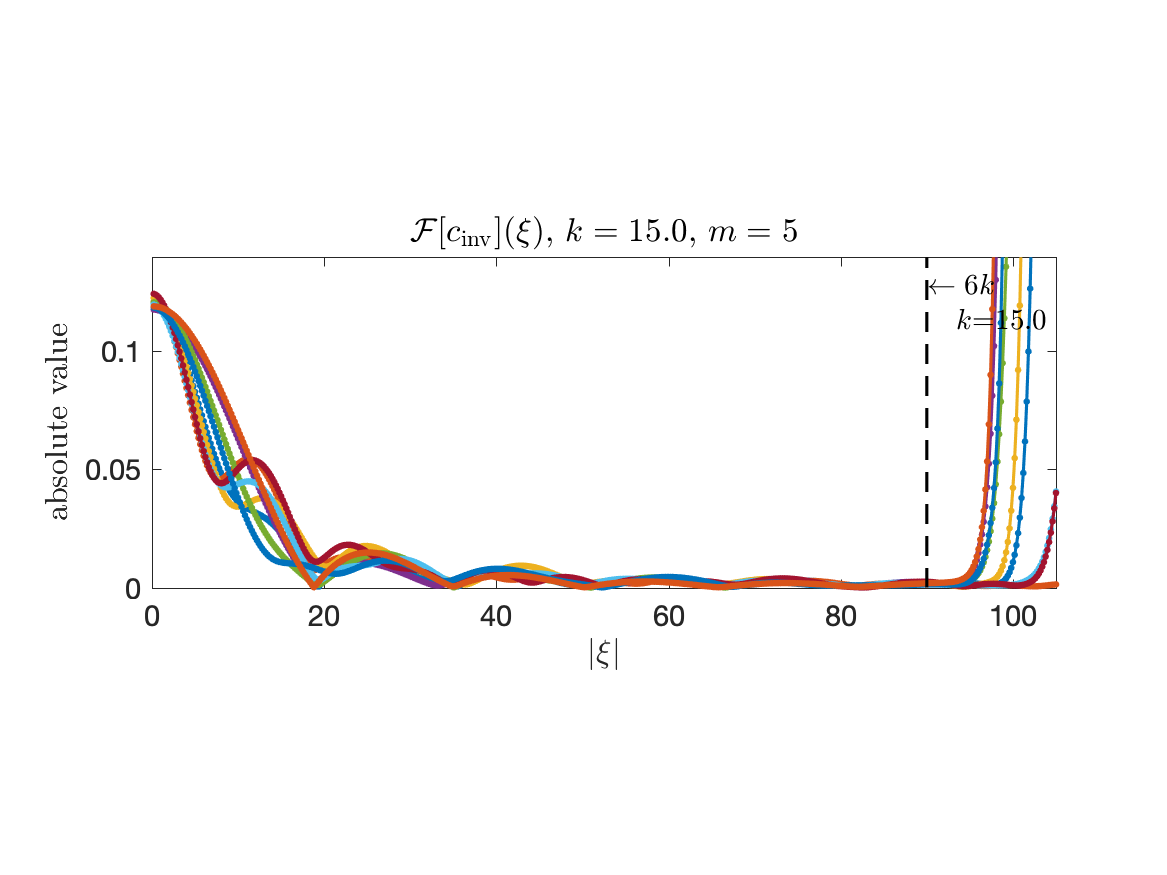
\includegraphics[width=0.54\textwidth,trim=10 60 30 90,clip]{./figs/pwc_5_Fc_0150.png}\\
\caption[算法2:不连续位势的重构结果]{当非线性次数$m=5$,波数\textbf{(i)} $k = 5$,\textbf{(ii)} $k = 10$和\textbf{(iii)} $k = 15$时的重构结果.
第一列:利用频域截断$|\xi| \leq (m+1)k$得到的重构位势函数$c_{\textrm{inv}}(x)$.
第二列:真实位势函数和重构位势函数的角度误差$|c(x) - c_{\textrm{inv}}(x)|$.
第三列:重构位势函数的傅立叶系数的绝对值$\mathcal{F}[c_{\textrm{inv}}](\xi)|$.
}
\label{fig:5_pwc}
\end{figure}

如果多个图形相互独立,并不共用一个图形计数器,那么用 \texttt{minipage} 或者
\texttt{parbox} 就可以,如图~\ref{fig:parallel1} 与图~\ref{fig:parallel2}。

\begin{figure}[H]
  \centering
  \begin{minipage}{0.48\textwidth}
    \centering
    
\includegraphics[height=1.5cm]{./figs/fudan-emblem.pdf}
    \caption{并排第一个图}
    \label{fig:parallel1}
  \end{minipage}\hfill
  \begin{minipage}{0.48\textwidth}
    \centering
    
\includegraphics[height=1.5cm]{./figs/fudan-emblem.pdf}
    \caption{并排第二个图}
    \label{fig:parallel2}
  \end{minipage}
\end{figure}

如果要为共用一个计数器的多个子图添加子图题,建议使用较新的 subcaption 宏包,不建议使用 subfigure 或 subfig 等宏包。

推荐使用 subcaption宏包的 subcaptionbox并排子图,子图题置于子图之下,子图号用 a)、b) 等表示。也可以使用subcaption宏包的 subcaption(放在 minipage中,用法同 caption)。

subcaption 宏包也提供了subfigure和 subtable 环境,如
图~\ref{fig:subfigure}。

\begin{figure}[!htp]
  \centering
  \begin{subfigure}{0.3\textwidth}
    \centering
    
\includegraphics[height=2cm]{./figs/fudan-emblem.pdf}
    \caption{校徽}
  \end{subfigure}
  \hspace{1cm}
  \begin{subfigure}{0.4\textwidth}
    \centering
    
\includegraphics[height=1.5cm]{./figs/fudan-emblem.pdf}
    \caption{校徽。这个图略矮些,subfigure中同一行的子图在顶端对齐。}
  \end{subfigure}
  \caption{包含子图题的范例(使用 subfigure)}
  \label{fig:subfigure}
\end{figure}

\subsection{Tik作图}
以下摘自Hansimov的知乎文章[LaTeX 绘图指南 - 001] TikZ 的简介、资源以及学习方法\footnote{https://zhuanlan.zhihu.com/p/48300815}。

TikZ 是 LaTeX 下的一个(著名的)绘图宏包。TikZ 的德文原文是 TikZ ist kein Zeichenprogramm, 这是一个 "GNU's Not Unix!" 式的递归缩写。翻译成英文就是 TikZ is not a drawing program,中文意思是“TikZ 不是一个绘图程序”。(程序员式冷幽默)

PGF/TikZ 相关的学习资源很多,可以参考这个项目:xiaohanyu/awesome-tikz\footnote{https://github.com/xiaohanyu/awesome-tikz}。基本列出了常见的高质资源,语言大多为英文。此外还有一些重要的资源:

\begin{itemize}
    \item 英文文档:pgfmanual\footnote{http://mirrors.ctan.org/graphics/pgf/base/doc/pgfmanual.pdf}
    \item PGF/TikZ 中文手册(在翻):pgfmanual-zh\footnote{https://github.com/Hansimov/pgfmanual-zh}
    \item 命令大全:VisualTikZ\footnote{http://mirrors.ctan.org/info/visualtikz/VisualTikZ.pdf}
     \item 各种样例:TikZ and PGF examples\footnote{http://www.texample.net/tikz/examples/all/}
     \item TeX 社区:Questions tagged [tikz-pgf]\footnote{https://tex.stackexchange.com/questions/tagged/tikz-pgf}
\end{itemize}

下面是来自于邹森博士论文中的一个样例。
\begin{figure}[H]
\centering
%----------------------%
% original, STYLE 1
\begin{tikzpicture}[>=latex,scale=1.0]
\draw[rounded corners=8,dashed,fill=gray!15!white]
 (0.6,-0.8) rectangle (2.6,0.8) node at ++(-0.3,-0.3) {$\Omega$};
\node  (f) at (0,0) {$f$};
\node  (u) at (2,0) {$u$};
\node (du) at (4,0) {$\partial_{\nu} u$};
\draw[->,thick,blue] (f) -- node[above] {$c$}  (u) node[pos=0.5,below] {\footnotesize$(I)$};
\draw[->,thick] (u) -- (du) node[pos=0.5,below] {\footnotesize$\partial_{\nu}$};
\draw[rounded corners=15,->,thick,blue] (f) |- (2,1.2) node[above] {$\Lambda_{c}$} -| (du);
\node at (2,-1.3) {\textbf{(i)} 原始问题};
\end{tikzpicture}%\\
%----------------------%
% linearized
\hspace{4ex}
\begin{tikzpicture}[>=latex,scale=1.0]
\draw[rounded corners=8,dashed,fill=gray!15!white]
 (0.5,-0.8) rectangle (4.6,0.8) node at ++(-0.3,-0.3) {$\Omega$};
\node   (f) at (0,0) {$f$};
\node  (u0) at (2,0) {$u^{(0)}$};
\node  (u1) at (4,0) {$u^{(1)}$};
\node (du1) at (6,0) {$\partial_{\nu} u^{(1)}$};
\draw[->,thick]  (f) --  (u0) node[pos=0.5,below] {\footnotesize$(I_{0})$};
\draw[->,thick,blue] (u0) -- node[above] {$c$}  (u1) node[pos=0.5,below] {\footnotesize$(I_{1})$};
\draw[->,thick] (u1) -- (du1) node[pos=0.5,below] {\footnotesize$\partial_{\nu}$};
\draw[rounded corners=15,->,thick,blue] (f) |- (3,1.2) node[above] {$\Lambda'_{c}$} -| (du1);
\node at (3,-1.3) {\textbf{(ii)} 线性化系统};
\end{tikzpicture}\\
%----------------------%
% PIE type
\vspace{1ex}
\begin{tikzpicture}[>=latex,scale=1.0]
\draw[rounded corners=8,dashed,fill=gray!15!white]
 (0.5,-1) rectangle (6.6,1) node at ++(-0.3,-0.3) {$\Omega$};
\node   (f) at (0,0) {$f_{j}$};
\draw[rounded corners=2,red] (-0.5,0.7) rectangle (2.45,-0.7) node at ++(-0.4,0.2) {\tiny$j \in S$};
\node  (u0) at (2,0) {$u_{j}^{(0)}$};
\node  (v0) at (4,0) {$u_{S}^{(0)}$};
\node  (v1) at (6,0) {$u_{S}^{(1)}$};
\node (dv1) at (8,0) {$\partial_{\nu} u_{S}^{(1)}$};
\draw[->,thick]  (f) --  (u0) node[pos=0.5,below] {\footnotesize$(I_{0})$};
\draw[->,thick,red] (u0) --  (v0) node[pos=0.5,below] {\footnotesize$\sum\limits_{j \in S}$};
\draw[->,thick,blue] (v0) -- node[above] {$c$}  (v1) node[pos=0.5,below] {\footnotesize$(I_{S}^{(1)})$};
\draw[->,thick] (v1) -- (dv1) node[pos=0.5,below] {\footnotesize$\partial_{\nu}$};
\draw[rounded corners=2] (-0.7,1.3) rectangle (8.7,-1.3) node at ++(-0.4,0.2) {\tiny$S \subseteq U$};
\draw[rounded corners=15,->,thick,blue] (f)++(0,0.7) |- (4,1.6) node[above] {$\Lambda'_{c}$} -| (dv1);
\node at (4,-1.8) {\textbf{(iii)} PIE型线性化系统};
\end{tikzpicture}
%----------------------%
\caption[Alessandrini等式示意图]{三种Alessandrini型等式的对比图示}
\label{fig:identity}
\end{figure}


\section{表格}

\subsection{基本表格}

编排表格应简单明了,表达一致,明晰易懂,表文呼应、内容一致。表题置于表上。

表格的编排建议采用国际通行的三线表\footnote{三线表,以其形式简洁、功能分明、阅读
方便而在科技论文中被推荐使用。三线表通常只有 3 条线,即顶线、底线和栏目线,没有竖线。}。三线表可以使用 booktabs 提供的 toprule、midrule 和bottomrule。它们与 longtable能很好的配合使用。

\begin{table}[!hpt]
  \caption[一个颇为标准的三线表]{一个颇为标准的三线表\footnotemark}
  \label{tab:firstone}
  \centering
  \begin{tabular}{@{}llr@{}} \toprule
    \multicolumn{2}{c}{Item} \\ \cmidrule(r){1-2}
    Animal & Description & Price (\$)\\ \midrule
    Gnat  & per gram  & 13.65 \\
          & each      & 0.01 \\
    Gnu   & stuffed   & 92.50 \\
    Emu   & stuffed   & 33.33 \\
    Armadillo & frozen & 8.99 \\ \bottomrule
  \end{tabular}
\end{table}
\subsection{复杂表格}

我们经常会在表格下方标注数据来源,或者对表格里面的条目进行解释。可以用threeparttable实现带有脚注的表格,如表~\ref{tab:footnote}。

\begin{table}[!htpb]
  \bicaption{一个带有脚注的表格的例子}{A Table with footnotes}
  \label{tab:footnote}
  \centering
  \begin{threeparttable}[b]
     \begin{tabular}{ccccccc}
      \toprule
      \multirow{2}*{total} & \multicolumn{2}{c}{20\tnote{a}} & \multicolumn{2}{c}{40} & \multicolumn{2}{c}{60} \\
      \cmidrule(lr){2-3}\cmidrule(lr){4-5}\cmidrule(lr){6-7}
      & www & \multicolumn{1}{c}{k} & www & k & www & k \\ % 使用说明符 d 的列会自动进入数学模式,使用 \multicolumn 对文字表头做特殊处理
      \midrule
      & $\underset{(2.12)}{4.22}$ & 120.0140\tnote{b} & 333.15 & 0.0411 & 444.99 & 0.1387 \\
      & 168.6123 & 10.86 & 255.37 & 0.0353 & 376.14 & 0.1058 \\
      & 6.761    & 0.007 & 235.37 & 0.0267 & 348.66 & 0.1010 \\
      \bottomrule
    \end{tabular}
    \begin{tablenotes}
    \item [a] the first note.
    \item [b] the second note.
    \end{tablenotes}
  \end{threeparttable}
\end{table}

如某个表需要转页接排,可以用longtable实现。接排时表题省略,表头应重复书
写,并在右上方写“续表 xx”,如表~\ref{tab:performance}。

\begin{ThreePartTable}
  \begin{TableNotes}
    \item[a] 一个脚注
    \item[b] 另一个脚注
  \end{TableNotes}
  \begin{longtable}[c]{c*{6}{r}}
    \bicaption{实验数据}{Experimental data}
    \label{tab:performance} \\
    \toprule
    测试程序 & \multicolumn{1}{c}{正常运行} & \multicolumn{1}{c}{同步}
      & \multicolumn{1}{c}{检查点} & \multicolumn{1}{c}{卷回恢复}
      & \multicolumn{1}{c}{进程迁移} & \multicolumn{1}{c}{检查点} \\
    & \multicolumn{1}{c}{时间 (s)} & \multicolumn{1}{c}{时间 (s)}
      & \multicolumn{1}{c}{时间 (s)} & \multicolumn{1}{c}{时间 (s)}
      & \multicolumn{1}{c}{时间 (s)} &  文件(KB)\\
    \midrule
    \endfirsthead
    \multicolumn{7}{l}{\textbf{续表~\thetable}} \\
    % 英语论文:\multicolumn{7}{r}{\textbf{Table~\thetable~(continued)}} \\
    \toprule
    测试程序 & \multicolumn{1}{c}{正常运行} & \multicolumn{1}{c}{同步}
      & \multicolumn{1}{c}{检查点} & \multicolumn{1}{c}{卷回恢复}
      & \multicolumn{1}{c}{进程迁移} & \multicolumn{1}{c}{检查点} \\
    & \multicolumn{1}{c}{时间 (s)} & \multicolumn{1}{c}{时间 (s)}
      & \multicolumn{1}{c}{时间 (s)} & \multicolumn{1}{c}{时间 (s)}
      & \multicolumn{1}{c}{时间 (s)}&  文件(KB)\\
    \midrule
    \endhead
    \hline
    \multicolumn{7}{r}{续下页}
    \endfoot
    \insertTableNotes
    \endlastfoot
    CG.A.2 & 23.05 & 0.002 & 0.116 & 0.035 & 0.589 & 32491 \\
    CG.A.4 & 15.06 & 0.003 & 0.067 & 0.021 & 0.351 & 18211 \\
    CG.A.8 & 13.38 & 0.004 & 0.072 & 0.023 & 0.210 & 9890 \\
    CG.B.2 & 867.45 & 0.002 & 0.864 & 0.232 & 3.256 & 228562 \\
    CG.B.4 & 501.61 & 0.003 & 0.438 & 0.136 & 2.075 & 123862 \\
    CG.B.8 & 384.65 & 0.004 & 0.457 & 0.108 & 1.235 & 63777 \\
    MG.A.2 & 112.27 & 0.002 & 0.846 & 0.237 & 3.930 & 236473 \\
    MG.A.4 & 59.84 & 0.003 & 0.442 & 0.128 & 2.070 & 123875 \\
    MG.A.8 & 31.38 & 0.003 & 0.476 & 0.114 & 1.041 & 60627 \\
    MG.B.2 & 526.28 & 0.002 & 0.821 & 0.238 & 4.176 & 236635 \\
    MG.B.4 & 280.11 & 0.003 & 0.432 & 0.130 & 1.706 & 123793 \\
    MG.B.8 & 148.29 & 0.003 & 0.442 & 0.116 & 0.893 & 60600 \\
    LU.A.2 & 2116.54 & 0.002 & 0.110 & 0.030 & 0.532 & 28754 \\
    LU.A.4 & 1102.50 & 0.002 & 0.069 & 0.017 & 0.255 & 14915 \\
    LU.A.8 & 574.47 & 0.003 & 0.067 & 0.016 & 0.192 & 8655 \\
    LU.B.2 & 9712.87 & 0.002 & 0.357 & 0.104 & 1.734 & 101975 \\
    LU.B.4 & 4757.80 & 0.003 & 0.190 & 0.056 & 0.808 & 53522 \\
    LU.B.8 & 2444.05 & 0.004 & 0.222 & 0.057 & 0.548 & 30134 \\
    EP.A.2 & 123.81 & 0.002 & 0.010 & 0.003 & 0.074 & 1834 \\
    EP.A.4 & 61.92 & 0.003 & 0.011 & 0.004 & 0.073 & 1743 \\
    EP.A.8 & 31.06 & 0.004 & 0.017 & 0.005 & 0.073 & 1661 \\
    EP.B.2 & 495.49 & 0.001 & 0.009 & 0.003 & 0.196 & 2011 \\
    EP.B.4 & 247.69 & 0.002 & 0.012 & 0.004 & 0.122 & 1663 \\
    EP.B.8 & 126.74 & 0.003 & 0.017 & 0.005 & 0.083 & 1656 \\
    SP.A.2 & 123.81 & 0.002 & 0.010 & 0.003 & 0.074 & 1854 \\
    SP.A.4 & 51.92 & 0.003 & 0.011 & 0.004 & 0.073 & 1543 \\
    SP.A.8 & 31.06 & 0.004 & 0.017 & 0.005 & 0.073 & 1671 \\
    SP.B.2 & 495.49 & 0.001 & 0.009 & 0.003 & 0.196 & 2411 \\
    SP.B.4 \tnote{a} & 247.69 & 0.002 & 0.014 & 0.006 & 0.152 & 2653 \\
    SP.B.8 \tnote{b} & 126.74 & 0.003 & 0.017 & 0.005 & 0.082 & 1755 \\
    \bottomrule
  \end{longtable}
\end{ThreePartTable}

\section{算法环境}

算法环境可以使用 agorithms宏包或者较新的algorithm2e实现。
算法~\ref{algo:algorithm} 是一个使用algorithm2e的例子。关于排版算法环境
的具体方法,请阅读相关宏包的官方文档。

\begin{algorithm}[htb]
  \caption{算法示例}
  \label{algo:algorithm}
  \small
  \SetAlgoLined
  \KwData{this text}
  \KwResult{how to write algorithm with \LaTeXe }

  initialization\;
  \While{not at end of this document}{
    read current\;
    \eIf{understand}{
      go to next section\;
      current section becomes this one\;
    }{
      go back to the beginning of current section\;
    }
  }
\end{algorithm}

同样可以考虑以如下表格的形式实现。
\begin{table}[H] 
\centering
\begin{tabular}{p{\textwidth}}
\toprule
\textbf{算法1:3维情况下部分边界观测反问题$\lambda_c\rightarrow c$的神经网络结构}  \\%
\midrule
\textbf{输入:} %
$\lambda\in\mathbb{R}^{N_{m_1}\times N_{m_2}\times N_{h_1}\times N_{h_2}}$,参数$channel,N_{z},w,n_{cnn}$;
\textbf{输出:} %
$c\in \mathbb{R}^{N_x\times N_y\times N_y}$. \\[-15pt]%
\begin{enumerate}[1:]
  \item 将$\lambda_c$的后两个维度向量化,形成一个三维张量,记为$\lambda$;
  \item $\tilde{\lambda}_{\hat{h}}\leftarrow\texttt{Encoding3d}[channel](\lambda)$; %
  \item  $\tilde{c}_{\hat{z}_3}\leftarrow\texttt{BCR-Net2d}(\tilde{\lambda}_{\hat{h}}) $; %
  \item $\bar{c}\leftarrow\texttt{Decoding3d}[N_z](\tilde{c}_{\hat{z_3}})$;%
  \item $c\leftarrow\texttt{CNN3d}[w,n_{cnn}](\bar{c})$;%
  \item 返回 $c$ %
\end{enumerate} \\%
\bottomrule
\end{tabular}
\caption*{算法 1: 线性薛定谔位势反问题的部分边界观测问题的神经网络结构\mycite{FY2020}}
\end{table}



